\documentclass{standalone}
\usepackage{tikz}
\usetikzlibrary{patterns, positioning}

\begin{document}
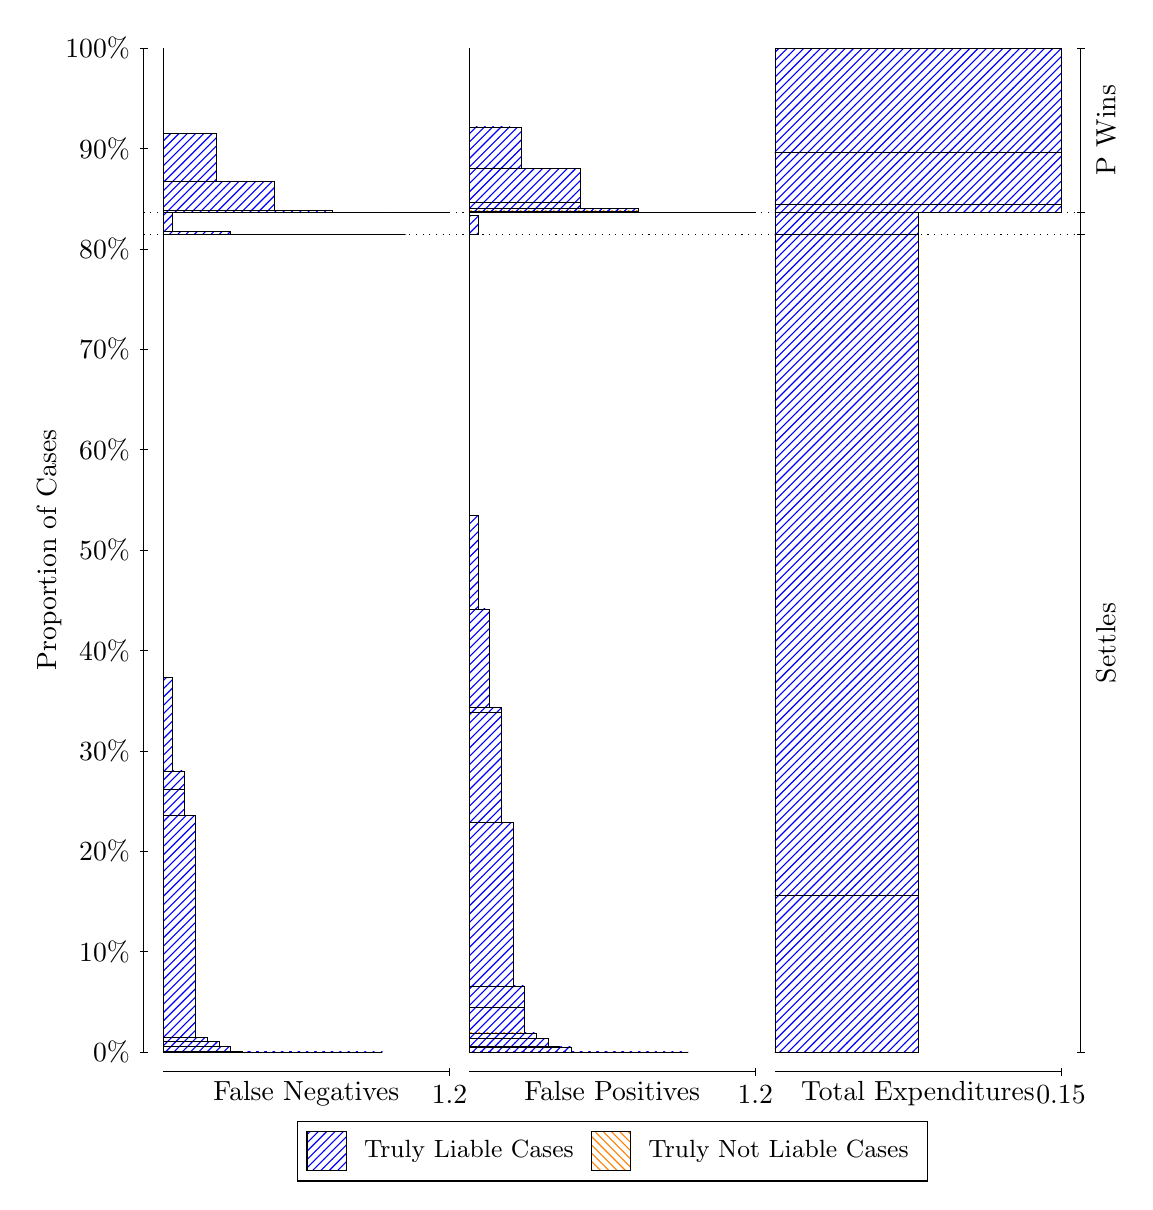
\begin{tikzpicture}
\draw[black, very thin] (1.5,1.75) -- (1.5,14.5);
\node[rotate=90, anchor=center] at (0.3, 8.125) {Proportion of Cases};
\draw[black, very thin] (1.45,1.75) -- (1.55,1.75);
\node[anchor=east] at (1.45, 1.75) {0\%};
\draw[black, very thin] (1.45,3.025) -- (1.55,3.025);
\node[anchor=east] at (1.45, 3.025) {10\%};
\draw[black, very thin] (1.45,4.3) -- (1.55,4.3);
\node[anchor=east] at (1.45, 4.3) {20\%};
\draw[black, very thin] (1.45,5.575) -- (1.55,5.575);
\node[anchor=east] at (1.45, 5.575) {30\%};
\draw[black, very thin] (1.45,6.85) -- (1.55,6.85);
\node[anchor=east] at (1.45, 6.85) {40\%};
\draw[black, very thin] (1.45,8.125) -- (1.55,8.125);
\node[anchor=east] at (1.45, 8.125) {50\%};
\draw[black, very thin] (1.45,9.4) -- (1.55,9.4);
\node[anchor=east] at (1.45, 9.4) {60\%};
\draw[black, very thin] (1.45,10.675) -- (1.55,10.675);
\node[anchor=east] at (1.45, 10.675) {70\%};
\draw[black, very thin] (1.45,11.95) -- (1.55,11.95);
\node[anchor=east] at (1.45, 11.95) {80\%};
\draw[black, very thin] (1.45,13.225) -- (1.55,13.225);
\node[anchor=east] at (1.45, 13.225) {90\%};
\draw[black, very thin] (1.45,14.5) -- (1.55,14.5);
\node[anchor=east] at (1.45, 14.5) {100\%};

\draw[black, very thin] (13.4,1.75) -- (13.4,14.5);
\draw[black, very thin] (13.35,1.75) -- (13.45,1.75);
\node[anchor=west] at (13.35, 1.75) {};
\draw[black, very thin] (13.35,12.136) -- (13.45,12.136);
\node[anchor=west] at (13.35, 12.136) {};
\draw[black, very thin] (13.35,12.416) -- (13.45,12.416);
\node[anchor=west] at (13.35, 12.416) {};
\draw[black, very thin] (13.35,14.5) -- (13.45,14.5);
\node[anchor=west] at (13.35, 14.5) {};

\draw[black, very thin, pattern color=blue, pattern=north east lines] (1.75,1.75) rectangle (4.5306,1.75);
\draw[black, very thin, pattern color=blue, pattern=north east lines] (1.75,1.75) rectangle (4.234,1.75);
\draw[black, very thin, pattern color=blue, pattern=north east lines] (1.75,1.75) rectangle (3.9374,1.75);
\draw[black, very thin, pattern color=blue, pattern=north east lines] (1.75,1.75) rectangle (3.7891,1.75);
\draw[black, very thin, pattern color=blue, pattern=north east lines] (1.75,1.75) rectangle (3.6408,1.75);
\draw[black, very thin, pattern color=blue, pattern=north east lines] (1.75,1.75) rectangle (3.4925,1.75);
\draw[black, very thin, pattern color=blue, pattern=north east lines] (1.75,1.75) rectangle (3.3442,1.75);
\draw[black, very thin, pattern color=blue, pattern=north east lines] (1.75,1.75) rectangle (3.1959,1.75);
\draw[black, very thin, pattern color=blue, pattern=north east lines] (1.75,1.75) rectangle (3.0476,1.75);
\draw[black, very thin, pattern color=blue, pattern=north east lines] (1.75,1.75) rectangle (2.8993,1.7506);
\draw[black, very thin, pattern color=blue, pattern=north east lines] (1.75,1.7506) rectangle (2.751,1.7551);
\draw[black, very thin, pattern color=blue, pattern=north east lines] (1.75,1.7551) rectangle (2.6027,1.8184);
\draw[black, very thin, pattern color=blue, pattern=north east lines] (1.75,1.8184) rectangle (2.4544,1.8834);
\draw[black, very thin, pattern color=blue, pattern=north east lines] (1.75,1.8834) rectangle (2.4544,1.8834);
\draw[black, very thin, pattern color=blue, pattern=north east lines] (1.75,1.8834) rectangle (2.3061,1.9387);
\draw[black, very thin, pattern color=blue, pattern=north east lines] (1.75,1.9387) rectangle (2.1578,4.7544);
\draw[black, very thin, pattern color=blue, pattern=north east lines] (1.75,4.7544) rectangle (2.0095,5.0923);
\draw[black, very thin, pattern color=blue, pattern=north east lines] (1.75,5.0923) rectangle (2.0095,5.3195);
\draw[black, very thin, pattern color=blue, pattern=north east lines] (1.75,5.3195) rectangle (1.8612,6.5085);
\draw[black, very thin, pattern color=orange, pattern=north west lines] (1.75,6.5085) rectangle (1.75,6.5085);
\draw[black, very thin, pattern color=blue, pattern=north east lines] (1.75,6.5085) rectangle (1.75,12.136);
\draw[black, very thin, pattern color=blue, pattern=north east lines] (1.75,12.136) rectangle (4.8272,12.136);
\draw[black, very thin, pattern color=blue, pattern=north east lines] (1.75,12.136) rectangle (4.0857,12.136);
\draw[black, very thin, pattern color=blue, pattern=north east lines] (1.75,12.136) rectangle (3.3442,12.136);
\draw[black, very thin, pattern color=blue, pattern=north east lines] (1.75,12.136) rectangle (2.6027,12.174);
\draw[black, very thin, pattern color=blue, pattern=north east lines] (1.75,12.174) rectangle (1.8612,12.416);
\draw[black, very thin, pattern color=orange, pattern=north west lines] (1.75,12.416) rectangle (1.75,12.416);
\draw[black, very thin, pattern color=blue, pattern=north east lines] (1.75,12.416) rectangle (5.3833,12.416);
\draw[black, very thin, pattern color=blue, pattern=north east lines] (1.75,12.416) rectangle (4.6418,12.416);
\draw[black, very thin, pattern color=blue, pattern=north east lines] (1.75,12.416) rectangle (3.9003,12.438);
\draw[black, very thin, pattern color=blue, pattern=north east lines] (1.75,12.438) rectangle (3.752,12.438);
\draw[black, very thin, pattern color=blue, pattern=north east lines] (1.75,12.438) rectangle (3.1588,12.807);
\draw[black, very thin, pattern color=blue, pattern=north east lines] (1.75,12.807) rectangle (3.0105,12.807);
\draw[black, very thin, pattern color=blue, pattern=north east lines] (1.75,12.807) rectangle (3.0105,12.807);
\draw[black, very thin, pattern color=blue, pattern=north east lines] (1.75,12.807) rectangle (2.4173,13.415);
\draw[black, very thin, pattern color=blue, pattern=north east lines] (1.75,13.415) rectangle (2.269,13.417);
\draw[black, very thin, pattern color=blue, pattern=north east lines] (1.75,13.417) rectangle (2.269,13.418);
\draw[black, very thin, pattern color=orange, pattern=north west lines] (1.75,13.418) rectangle (1.75,13.418);
\draw[black, very thin, pattern color=blue, pattern=north east lines] (1.75,13.418) rectangle (1.75,14.5);
\draw[black, very thin, pattern color=orange, pattern=north west lines] (5.6333,1.75) rectangle (8.4139,1.75);
\draw[black, very thin, pattern color=blue, pattern=north east lines] (5.6333,1.75) rectangle (8.4139,1.75);
\draw[black, very thin, pattern color=orange, pattern=north west lines] (5.6333,1.75) rectangle (8.1173,1.75);
\draw[black, very thin, pattern color=blue, pattern=north east lines] (5.6333,1.75) rectangle (8.1173,1.75);
\draw[black, very thin, pattern color=orange, pattern=north west lines] (5.6333,1.75) rectangle (7.8207,1.75);
\draw[black, very thin, pattern color=blue, pattern=north east lines] (5.6333,1.75) rectangle (7.8207,1.75);
\draw[black, very thin, pattern color=blue, pattern=north east lines] (5.6333,1.75) rectangle (7.6724,1.75);
\draw[black, very thin, pattern color=orange, pattern=north west lines] (5.6333,1.75) rectangle (7.5241,1.75);
\draw[black, very thin, pattern color=blue, pattern=north east lines] (5.6333,1.75) rectangle (7.5241,1.75);
\draw[black, very thin, pattern color=blue, pattern=north east lines] (5.6333,1.75) rectangle (7.3759,1.7501);
\draw[black, very thin, pattern color=orange, pattern=north west lines] (5.6333,1.7501) rectangle (7.2276,1.7501);
\draw[black, very thin, pattern color=blue, pattern=north east lines] (5.6333,1.7501) rectangle (7.2276,1.7502);
\draw[black, very thin, pattern color=blue, pattern=north east lines] (5.6333,1.7502) rectangle (7.0793,1.7508);
\draw[black, very thin, pattern color=orange, pattern=north west lines] (5.6333,1.7508) rectangle (6.931,1.7508);
\draw[black, very thin, pattern color=blue, pattern=north east lines] (5.6333,1.7508) rectangle (6.931,1.8159);
\draw[black, very thin, pattern color=blue, pattern=north east lines] (5.6333,1.8159) rectangle (6.7827,1.8183);
\draw[black, very thin, pattern color=blue, pattern=north east lines] (5.6333,1.8183) rectangle (6.6344,1.8183);
\draw[black, very thin, pattern color=orange, pattern=north west lines] (5.6333,1.8183) rectangle (6.6344,1.8183);
\draw[black, very thin, pattern color=blue, pattern=north east lines] (5.6333,1.8183) rectangle (6.6344,1.9254);
\draw[black, very thin, pattern color=blue, pattern=north east lines] (5.6333,1.9254) rectangle (6.4861,1.9918);
\draw[black, very thin, pattern color=orange, pattern=north west lines] (5.6333,1.9918) rectangle (6.3378,1.9918);
\draw[black, very thin, pattern color=blue, pattern=north east lines] (5.6333,1.9918) rectangle (6.3378,2.3119);
\draw[black, very thin, pattern color=blue, pattern=north east lines] (5.6333,2.3119) rectangle (6.3378,2.5881);
\draw[black, very thin, pattern color=blue, pattern=north east lines] (5.6333,2.5881) rectangle (6.1895,4.6693);
\draw[black, very thin, pattern color=orange, pattern=north west lines] (5.6333,4.6693) rectangle (6.0412,4.6693);
\draw[black, very thin, pattern color=blue, pattern=north east lines] (5.6333,4.6693) rectangle (6.0412,6.0587);
\draw[black, very thin, pattern color=blue, pattern=north east lines] (5.6333,6.0587) rectangle (6.0412,6.1224);
\draw[black, very thin, pattern color=blue, pattern=north east lines] (5.6333,6.1224) rectangle (5.8929,6.1224);
\draw[black, very thin, pattern color=blue, pattern=north east lines] (5.6333,6.1224) rectangle (5.8929,7.3772);
\draw[black, very thin, pattern color=blue, pattern=north east lines] (5.6333,7.3772) rectangle (5.7446,8.5663);
\draw[black, very thin, pattern color=blue, pattern=north east lines] (5.6333,8.5663) rectangle (5.6333,12.136);
\draw[black, very thin, pattern color=orange, pattern=north west lines] (5.6333,12.136) rectangle (5.7446,12.136);
\draw[black, very thin, pattern color=blue, pattern=north east lines] (5.6333,12.136) rectangle (5.7446,12.378);
\draw[black, very thin, pattern color=blue, pattern=north east lines] (5.6333,12.378) rectangle (5.6333,12.416);
\draw[black, very thin, pattern color=orange, pattern=north west lines] (5.6333,12.416) rectangle (9.2667,12.416);
\draw[black, very thin, pattern color=blue, pattern=north east lines] (5.6333,12.416) rectangle (9.2667,12.416);
\draw[black, very thin, pattern color=blue, pattern=north east lines] (5.6333,12.416) rectangle (8.5252,12.416);
\draw[black, very thin, pattern color=orange, pattern=north west lines] (5.6333,12.416) rectangle (8.5252,12.416);
\draw[black, very thin, pattern color=blue, pattern=north east lines] (5.6333,12.416) rectangle (8.5252,12.417);
\draw[black, very thin, pattern color=blue, pattern=north east lines] (5.6333,12.417) rectangle (7.7837,12.431);
\draw[black, very thin, pattern color=orange, pattern=north west lines] (5.6333,12.431) rectangle (7.7837,12.431);
\draw[black, very thin, pattern color=blue, pattern=north east lines] (5.6333,12.431) rectangle (7.7837,12.46);
\draw[black, very thin, pattern color=blue, pattern=north east lines] (5.6333,12.46) rectangle (7.0422,12.54);
\draw[black, very thin, pattern color=orange, pattern=north west lines] (5.6333,12.54) rectangle (7.0422,12.54);
\draw[black, very thin, pattern color=blue, pattern=north east lines] (5.6333,12.54) rectangle (7.0422,12.975);
\draw[black, very thin, pattern color=orange, pattern=north west lines] (5.6333,12.975) rectangle (6.8939,12.975);
\draw[black, very thin, pattern color=blue, pattern=north east lines] (5.6333,12.975) rectangle (6.8939,12.975);
\draw[black, very thin, pattern color=blue, pattern=north east lines] (5.6333,12.975) rectangle (6.3007,12.978);
\draw[black, very thin, pattern color=blue, pattern=north east lines] (5.6333,12.978) rectangle (6.3007,13.493);
\draw[black, very thin, pattern color=orange, pattern=north west lines] (5.6333,13.493) rectangle (6.1524,13.493);
\draw[black, very thin, pattern color=blue, pattern=north east lines] (5.6333,13.493) rectangle (6.1524,13.498);
\draw[black, very thin, pattern color=orange, pattern=north west lines] (5.6333,13.498) rectangle (5.6333,13.498);
\draw[black, very thin, pattern color=blue, pattern=north east lines] (5.6333,13.498) rectangle (5.6333,14.5);
\draw[black, very thin, pattern color=orange, pattern=north west lines] (9.5167,1.75) rectangle (11.333,1.75);
\draw[black, very thin, pattern color=blue, pattern=north east lines] (9.5167,1.75) rectangle (11.333,3.7395);
\draw[black, very thin, pattern color=orange, pattern=north west lines] (9.5167,3.7395) rectangle (11.333,3.7395);
\draw[black, very thin, pattern color=blue, pattern=north east lines] (9.5167,3.7395) rectangle (11.333,12.136);
\draw[black, very thin, pattern color=orange, pattern=north west lines] (9.5167,12.136) rectangle (11.333,12.136);
\draw[black, very thin, pattern color=blue, pattern=north east lines] (9.5167,12.136) rectangle (11.333,12.416);
\draw[black, very thin, pattern color=orange, pattern=north west lines] (9.5167,12.416) rectangle (13.15,12.416);
\draw[black, very thin, pattern color=blue, pattern=north east lines] (9.5167,12.416) rectangle (13.15,12.513);
\draw[black, very thin, pattern color=orange, pattern=north west lines] (9.5167,12.513) rectangle (13.15,12.513);
\draw[black, very thin, pattern color=blue, pattern=north east lines] (9.5167,12.513) rectangle (13.15,13.176);
\draw[black, very thin, pattern color=orange, pattern=north west lines] (9.5167,13.176) rectangle (13.15,13.176);
\draw[black, very thin, pattern color=blue, pattern=north east lines] (9.5167,13.176) rectangle (13.15,14.5);
\draw[black, dotted] (1.5,12.136) -- (13.4,12.136);
\draw[black, dotted] (1.5,12.416) -- (13.4,12.416);
\draw[black, very thin] (1.75,1.5) -- (5.3833,1.5);
\node[anchor=north] at (3.5667, 1.5) {False Negatives};
\draw[black, very thin] (5.3833,1.45) -- (5.3833,1.55);
\node[anchor=north] at (5.3833, 1.45) {1.2};

\draw[black, very thin] (5.6333,1.5) -- (9.2667,1.5);
\node[anchor=north] at (7.45, 1.5) {False Positives};
\draw[black, very thin] (9.2667,1.45) -- (9.2667,1.55);
\node[anchor=north] at (9.2667, 1.45) {1.2};

\draw[black, very thin] (9.5167,1.5) -- (13.15,1.5);
\node[anchor=north] at (11.333, 1.5) {Total Expenditures};
\draw[black, very thin] (13.15,1.45) -- (13.15,1.55);
\node[anchor=north] at (13.15, 1.45) {0.15};

\node[black, centered, rotate=90] at (13.72, 6.9429) {Settles};

\node[black, centered, rotate=90] at (13.72, 13.458) {P Wins};

\draw (7.449999999999999,1.5) node[draw=none] (baseCoordinate) {};
\begin{scope}[align=center]
        \matrix[scale=0.5, draw=black, below=0.5cm of baseCoordinate, nodes={draw}, column sep=0.1cm]{
            \node[rectangle, draw, minimum width=0.5cm, minimum height=0.5cm, pattern=north east lines, pattern color=blue] {}; &
            \node[draw=none, font=\small] (B) {Truly Liable Cases}; &
            \node[rectangle, draw, minimum width=0.5cm, minimum height=0.5cm, pattern=north west lines, pattern color=orange] {}; &
            \node[draw=none, font=\small] (B) {Truly Not Liable Cases}; \\
            };
\end{scope}

\end{tikzpicture}
\end{document}